\documentclass[UTF8,a4paper,11pt]{ctexart}

\usepackage{geometry}
\geometry{left=2.35cm,right=2.35cm,top=2.45cm,bottom=2.45cm}
\usepackage{graphicx}
\usepackage{float}
\usepackage{booktabs}
\usepackage{array}
\usepackage{xcolor}
\usepackage{hyperref}
\usepackage{caption}
\usepackage{tikz}
\usepackage{etoolbox}
\usetikzlibrary{arrows.meta,positioning,shapes.geometric}

\hypersetup{
  colorlinks=true,
  linkcolor=blue!50!black,
  urlcolor=blue!50!black,
  citecolor=blue!50!black
}

\pdfstringdefDisableCommands{%
  \def\unhbox#1{}%
  \def\kern{}%
}

\setlength{\parindent}{2em}
\setlength{\parskip}{0.28em}
\setlength{\emergencystretch}{3em}
\renewcommand{\arraystretch}{1.12}
\setlength{\tabcolsep}{4pt}
\graphicspath{{./}}

\title{北斗定位解算全流程软件系统开发实验报告}
\author{电子科学与技术专业实验}
\date{2026年5月}

\begin{document}
\maketitle
\begin{center}
\textbf{项目 GitHub 仓库：}\\
\url{https://github.com/tortrixx/beidou-positioning-experiment}
\end{center}
\tableofcontents
\newpage

\section{设计报告}

\subsection{需求分析}

本系统面向北斗/GNSS 伪距单点定位实验，设计目标是基于 RINEX 观测文件和广播星历文件，完成从数据导入、卫星位置计算、误差改正、定位解算到结果输出的完整软件流程。系统既要能够通过命令行完成批量解算，也要提供 PyQt 图形界面，便于进行文件选择、参数设置、实时结果查看和轨迹回放。

从实验任务看，系统需要解决的核心问题不是单独完成某一个算法函数，而是把 GNSS 定位中的多个环节串成稳定的数据处理链路。输入端需要兼容普通 RINEX 观测文件和导航文件；算法端需要根据广播星历计算 GPS/BDS 卫星位置、钟差和传播延迟改正；解算端需要根据伪距观测方程迭代求解接收机坐标；输出端需要生成 CSV、误差统计和可视化图像，供后续检查和报告使用。

结合实验文档中的五个核心模块，系统功能需求归纳如下：

\begin{enumerate}
\item 支持 RINEX 观测文件与导航文件解析，提取卫星编号、伪距、信噪比、广播星历参数和测站近似坐标。
\item 基于广播星历手写实现 GPS/BDS 卫星位置计算、卫星钟差修正、相对论效应修正、对流层与电离层延迟改正。
\item 构建伪距定位观测方程，采用迭代最小二乘解算接收机 ECEF 坐标、经纬高坐标和接收机钟差。
\item 支持连续历元定位分析，输出定位轨迹、误差统计、DOP 和卫星可见数变化。
\item 提供命令行与 PyQt GUI 两类入口，实现数据导入、参数设置、实时显示、绘图和轨迹回放。
\end{enumerate}

设计时还需要考虑以下约束。第一，核心定位算法由项目代码手写实现，不调用 RTKLIB、georinex、pymap3d 等现成定位库，第三方依赖主要用于 GUI、绘图和基础运行环境。第二，数据文件可能来自不同 RINEX 版本和不同 GNSS 系统，因此解析模块和解算模块之间需要通过统一数据结构连接。第三，实际数据中可能出现缺少星历、伪距无效、卫星数不足、参数设置错误等情况，系统需要给出可追踪的处理方式，而不是直接中断整个流程。

\subsection{功能设计}

\subsubsection{总体设计思路}

系统采用分层和模块化设计。底层负责 RINEX 文件读取与数据结构封装，中间层负责卫星位置、钟差和传播延迟改正，核心层负责单历元最小二乘定位，流程层负责连续历元循环、结果统计和绘图，最外层提供命令行脚本和 GUI 调用入口。

这种设计方式的主要考虑是让算法模块和界面模块分开。命令行脚本、批量运行脚本和 GUI 都调用同一套解析、修正和定位函数，避免出现“命令行一套逻辑、界面一套逻辑”的情况。后续如果增加新的数据集或新的结果展示方式，也可以尽量复用已有解算流程。

\subsubsection{功能模块划分}

软件按照实验要求划分为五个模块，各模块职责如表 \ref{tab:software-modules} 所示。模块之间的主调用关系为：RINEX 数据解析模块先生成观测历元和星历记录；卫星位置与修正模块根据观测时间和广播星历计算改正后的观测量；单点定位模块完成坐标解算；连续定位模块负责多历元循环和结果保存；系统整合测试模块提供 CLI、GUI 和批量运行入口。

\begin{table}[H]
\centering
\small
\begin{tabular}{p{0.18\linewidth}p{0.24\linewidth}p{0.48\linewidth}}
\toprule
模块 & 主要文件 & 功能说明 \\
\midrule
RINEX 数据解析 & \texttt{rinex\_obs.py}, \texttt{rinex\_nav.py} & 读取 OBS/NAV 文件，解析观测类型、历元数据、伪距、SNR、星历和电离层参数。 \\
卫星位置与修正 & \texttt{satellite.py}, \texttt{atmosphere.py} & 根据广播星历计算卫星 ECEF 坐标、钟差、相对论项、TGD、对流层和电离层改正。 \\
单点定位解算 & \texttt{positioning.py}, \texttt{coords.py} & 构建伪距方程，执行加权迭代最小二乘，输出 ECEF、BLH、PDOP、GDOP 和残差。 \\
连续定位分析 & \texttt{pipeline.py}, \texttt{analysis.py}, \texttt{plotting.py} & 逐历元循环解算，生成 CSV、误差统计、误差曲线、卫星数曲线和轨迹图。 \\
系统整合测试 & \texttt{experiment\_modules.py}, \texttt{scripts/} & 封装五个实验模块，提供 CLI、GUI、批量运行和模型训练入口。 \\
\bottomrule
\end{tabular}
\caption{软件功能模块划分}
\label{tab:software-modules}
\end{table}

\subsubsection{软件架构图}

系统总体架构如图 \ref{fig:software-architecture} 所示。数据从 RINEX 观测文件和导航文件进入后，先经过解析和预处理，再进入卫星位置、钟差和传播延迟改正模块。单点定位模块输出单历元解算结果，连续定位模块进一步生成结果文件和图像，最终由命令行或 GUI 展示。

\begin{figure}[H]
\centering
\resizebox{0.96\linewidth}{!}{%
\begin{tikzpicture}[
  node distance=0.42cm,
  stage/.style={draw, rounded corners, align=center, text width=2.5cm, minimum height=1.05cm, fill=blue!5},
  arrow/.style={-Latex, thick}
]
\node[stage] (a) {RINEX\\OBS/NAV};
\node[stage, right=of a] (b) {数据解析\\与预处理};
\node[stage, right=of b] (c) {卫星位置\\钟差与延迟改正};
\node[stage, right=of c] (d) {SPP\\最小二乘解算};
\node[stage, right=of d] (e) {连续定位\\误差分析};
\node[stage, right=of e] (f) {CSV/图像\\GUI 展示};
\foreach \x/\y in {a/b,b/c,c/d,d/e,e/f}
  \draw[arrow] (\x) -- (\y);
\end{tikzpicture}}
\caption{北斗定位解算软件总体架构}
\label{fig:software-architecture}
\end{figure}

\subsubsection{主要流程图}

定位解算的主要处理流程如图 \ref{fig:positioning-flow} 所示。流程中先完成文件读取和观测预处理，再对每颗可用卫星计算位置和误差改正，最后构建线性化伪距方程并通过迭代最小二乘求解。连续定位时，该流程会按设定步长在多个历元上重复执行。

\begin{figure}[H]
\centering
\begin{tikzpicture}[
  node distance=0.62cm,
  flow/.style={draw, rounded corners, align=center, text width=10.2cm, minimum height=0.62cm, fill=green!4},
  arrow/.style={-Latex, thick}
]
\node[flow] (a) {选择 RINEX 观测文件和导航文件};
\node[flow, below=of a] (b) {解析头文件、历元观测值、广播星历和电离层参数};
\node[flow, below=of b] (c) {剔除无效伪距、不健康卫星、无星历卫星和低高度角卫星};
\node[flow, below=of c] (d) {计算卫星 ECEF 坐标、卫星钟差、地球自转与传播延迟改正};
\node[flow, below=of d] (e) {构建伪距观测方程，按高度角设置权重};
\node[flow, below=of e] (f) {迭代最小二乘求解接收机坐标与钟差};
\node[flow, below=of f] (g) {输出 BLH、PDOP、GDOP、残差和有效卫星数};
\node[flow, below=of g] (h) {连续历元循环，生成 CSV、误差统计和图像};
\foreach \x/\y in {a/b,b/c,c/d,d/e,e/f,f/g,g/h}
  \draw[arrow] (\x) -- (\y);
\end{tikzpicture}
\caption{定位解算全流程}
\label{fig:positioning-flow}
\end{figure}

\subsubsection{数据结构设计}

项目主要数据结构定义在 \texttt{src/models.py} 中。设计时将观测文件、导航文件和定位结果分别封装，避免不同模块直接依赖原始文本文件格式。

\begin{table}[H]
\centering
\small
\begin{tabular}{p{0.28\linewidth}p{0.62\linewidth}}
\toprule
数据结构 & 设计作用 \\
\midrule
\texttt{ObsHeader} & 保存观测文件版本、测站名、近似坐标、观测类型和时间系统。 \\
\texttt{ObsEpoch} & 保存单历元时间、历元标志和以卫星编号为键的观测值字典。 \\
\texttt{NavRecord} & 保存单颗卫星的一组广播星历参数，包括轨道参数、钟差参数、TGD 和健康状态。 \\
\texttt{NavHeader} & 保存导航文件头信息，包括 GPS/BDS 电离层参数和闰秒信息。 \\
\texttt{PositionSolution} & 保存定位结果、接收机钟差、使用卫星数、DOP 和残差诊断指标。 \\
\bottomrule
\end{tabular}
\caption{核心数据结构设计}
\label{tab:data-structures}
\end{table}

这些结构将 RINEX 文件、卫星计算和定位结果解耦，使各模块之间通过明确的数据对象传递信息，便于调试和后续扩展。例如连续定位模块不需要直接解析 RINEX 文本，而是逐历元读取 \texttt{ObsEpoch}；绘图模块也不直接参与定位计算，只读取已经输出的 CSV 结果。

\subsubsection{输入输出与接口设计}

系统对外提供命令行和 GUI 两类接口。命令行入口主要用于复现、批量运行和自动化测试，典型脚本包括 \texttt{scripts/run\_spp.py}、\texttt{scripts/run\_continuous.py}、\texttt{scripts/run\_batch.py} 和 \texttt{scripts/plot\_results.py}。主要输入参数包括观测文件路径、导航文件路径、GNSS 系统类型、最大历元数、历元步长、输出 CSV 路径和图片保存目录。

GUI 入口由 \texttt{scripts/gui\_app.py} 提供，面向交互式演示。界面需要支持观测文件和导航文件选择、系统类型选择、最大历元数和高度角等参数设置，并显示最新定位坐标、使用卫星数、PDOP 和运行状态。运行完成后，GUI 通过绘图和轨迹回放功能查看结果。

输出文件按用途分为三类。第一类是连续定位 CSV，保存每个历元的时间、坐标、误差、DOP、卫星数和残差指标；第二类是汇总表，如 \texttt{results/summary.csv}，用于对不同数据集结果进行比较；第三类是图像文件，包括误差/DOP/卫星数曲线和轨迹散点图。这样的输出设计便于命令行、GUI 和报告图表共用同一批结果。

\subsubsection{异常处理与边界条件设计}

实际 GNSS 数据处理中，经常会遇到观测值缺失、星历不匹配或参数设置不合理的情况。系统在设计上将这些问题放在数据预处理和定位入口处处理，尽量避免错误向后传递。

\begin{enumerate}
\item 当某颗卫星没有有效伪距、星历缺失或健康状态不满足要求时，该卫星不参与当前历元定位。
\item 当卫星高度角低于阈值时，系统剔除该观测，以减小低高度角多路径和大气误差影响。
\item 当可用卫星数不足以构建定位方程时，当前历元不输出有效定位解，但连续定位流程继续处理后续历元。
\item 当步长、最大迭代次数等输入参数不合理时，入口脚本或 GUI 应先给出提示，避免出现除零或无意义循环。
\item 当遇到 Hatanaka 压缩文件等暂不支持格式时，系统识别后提示先转换为普通 RINEX，而不是直接按普通文本解析。
\end{enumerate}

通过这些边界处理，系统可以区分“文件无法解析”“当前历元无法定位”和“定位结果可用但精度较差”等不同情况，便于调试和结果解释。

\subsubsection{可扩展性设计}

当前系统重点支持 GPS、BDS 和 GPS+BDS 联合解算。为了便于后续扩展，系统在设计时尽量避免把系统类型写死在单一函数中，而是通过卫星编号、时间系统和导航记录选择对应处理逻辑。后续如果增加 Galileo、GLONASS 等系统，可以在现有 GNSS 系统识别、导航解析和钟差模型基础上继续扩展。

算法层也保留了继续改进的空间。例如，现有系统使用广播星历和伪距单点定位模型，后续可以进一步引入精密星历、更多电离层/对流层模型、鲁棒估计或动态滤波。界面层与算法层分离后，新增算法功能时不需要重写 GUI，只需要在参数设置和结果展示部分增加相应入口。

\newpage
\section{实验报告}

\subsection{实验目的}

本实验围绕北斗/GNSS 卫星导航定位原理，完成从 RINEX 数据读取到定位结果分析的软件开发流程。实验任务包括：解析 RINEX 观测与导航文件，计算卫星位置与卫星钟差，完成传播延迟修正，利用伪距观测方程进行单点定位，并对连续历元定位结果进行精度评估和可视化展示。

完成该实验需要掌握 RINEX 数据格式、广播星历轨道计算、GPS/BDT 时间系统、ECEF 与 BLH 坐标转换、最小二乘估计、DOP 指标、对流层和电离层延迟模型，以及 Python 模块化编程、PyQt GUI 编程和 Matplotlib 可视化方法。

\subsection{实验方法和步骤}

实验采用 Python 编写完整软件系统，主要步骤如下：

\begin{enumerate}
\item 导入 RINEX 观测文件和导航文件，读取测站近似坐标、观测类型、历元数据和广播星历。
\item 对观测数据进行预处理，剔除无效伪距、不健康卫星、无星历卫星和低高度角卫星。
\item 根据广播星历计算卫星 ECEF 坐标，完成轨道摄动修正、卫星钟差修正、相对论效应修正和 TGD 改正。
\item 使用 Saastamoinen 模型进行对流层延迟改正，使用 Klobuchar 模型进行 GPS/BDS 电离层延迟改正。
\item 构建伪距定位观测方程，采用加权迭代最小二乘求解接收机位置和钟差。
\item 将 ECEF 坐标转换为经纬高坐标，计算 PDOP、GDOP、残差 RMS 和最大残差。
\item 对连续历元重复解算，输出 CSV 结果、误差统计、误差曲线、DOP 曲线、卫星数曲线和轨迹散点图。
\item 使用 GUI 验证数据导入、参数设置、实时显示、绘图和轨迹回放功能。
\end{enumerate}

\subsection{实验软件总体设计}

软件采用模块化设计，将全流程拆分为数据解析、卫星修正、定位解算、连续分析和系统界面五部分。各模块之间通过统一的数据结构传递信息，既可以通过命令行单独运行，也可以由 GUI 调用完整流程。

\begin{figure}[H]
\centering
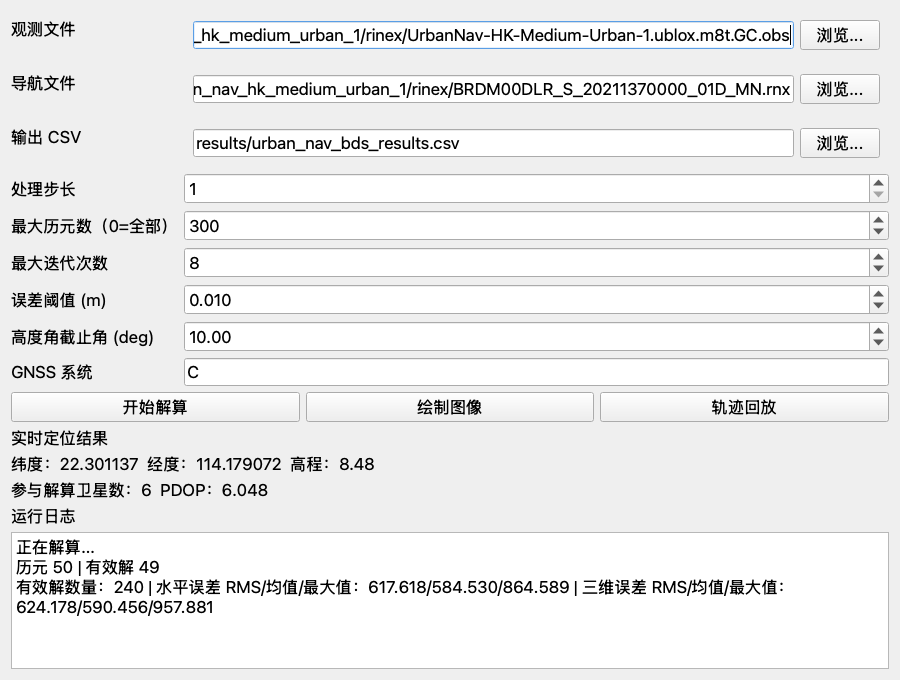
\includegraphics[width=0.82\linewidth]{figures/gui_main_window.png}
\caption{PyQt GUI 主界面}
\end{figure}

GUI 界面支持选择观测文件、导航文件和输出 CSV，设置步长、最大历元、最大迭代次数、误差阈值、高度角和 GNSS 系统。运行过程中显示最新纬度、经度、高程、使用卫星数和 PDOP；运行完成后可查看误差图并回放轨迹。

\subsection{详细设计及实现}

\subsubsection{RINEX 数据解析}

观测文件解析器支持 RINEX 2.11 与 RINEX 3。RINEX 2.11 通过 \texttt{\# / TYPES OF OBSERV} 读取观测类型；RINEX 3 通过 \texttt{SYS / \# / OBS TYPES} 分系统读取观测类型。程序按历元组织每颗卫星的观测值，保存伪距、载波相位、SNR 等信息。

导航文件解析器将广播星历保存为 \texttt{NavRecord}，包括半长轴平方根、偏心率、倾角、升交点赤经、近地点角、钟差参数、TGD 和健康状态等。对于 RINEX 3 mixed 导航文件，程序还能解析 \texttt{GPSA/GPSB/BDSA/BDSB} 电离层参数。

\subsubsection{卫星位置、钟差和传播延迟修正}

卫星位置计算基于广播星历公式。程序先计算平均角速度、平近点角、偏近点角和真近点角，再使用 \texttt{cuc/cus/crc/crs/cic/cis} 修正升交角距、轨道半径和倾角，最终转换到 ECEF 坐标系。BDS 使用 BDT 时间系统，程序在 mixed 数据中处理 GPST 到 BDT 的时间转换；BDS GEO 卫星 C01--C05 使用专门的 GEO 坐标转换分支。

卫星钟差采用钟差多项式、相对论项和 TGD 改正：

\begin{verbatim}
dt_sv = af0 + af1 * dt + af2 * dt^2 + relativistic - tgd
\end{verbatim}

传播延迟方面，对流层使用 Saastamoinen 模型，电离层使用 Klobuchar 模型。修正后的伪距进入定位方程。

\subsubsection{单点定位解算}

定位方程线性化后，采用迭代加权最小二乘求解。权重根据卫星高度角设置：

\begin{verbatim}
w = max(sin(elevation)^2, 0.05)
\end{verbatim}

GPS+BDS 联合定位时，状态向量为每个系统设置独立接收机钟差，避免 GPS 与 BDS 系统时间差被错误合并：

\begin{verbatim}
[dx, dy, dz, clock_G, clock_C]
\end{verbatim}

解算结束后输出 ECEF、BLH、接收机钟差、PDOP、GDOP、残差 RMS、最大残差和使用卫星数。

\subsubsection{连续定位、测试和可视化}

连续定位模块逐历元调用单点定位函数，并以 RINEX 头文件中的近似测站坐标作为参考，计算 ENU 方向误差、水平误差和三维误差。测试使用 UrbanNav、TWTF 等多组数据，覆盖城市动态 BDS、固定站 BDS 和 GPS+BDS 组合解算。

\begin{table}[H]
\centering
\small
\begin{tabular}{lccccc}
\toprule
数据集 & 系统 & 历元数 & 水平 RMS/m & 三维 RMS/m & PDOP 均值 \\
\midrule
UrbanNav & BDS & 240 & 617.618 & 624.178 & 6.575 \\
TWTF & BDS & 300 & 1.371 & 6.526 & 4.703 \\
TWTF & GPS+BDS & 300 & 1.208 & 2.936 & 2.755 \\
\bottomrule
\end{tabular}
\caption{重新运行后的北斗与 GPS+BDS 定位精度测试结果}
\end{table}

\begin{figure}[H]
\centering
\begin{minipage}{0.48\linewidth}
\centering

\includegraphics[width=\linewidth]{figures/urban_nav_bds_final/error_dop.png}
\caption*{(a) UrbanNav BDS 误差/DOP/卫星数曲线}
\end{minipage}
\hfill
\begin{minipage}{0.48\linewidth}
\centering
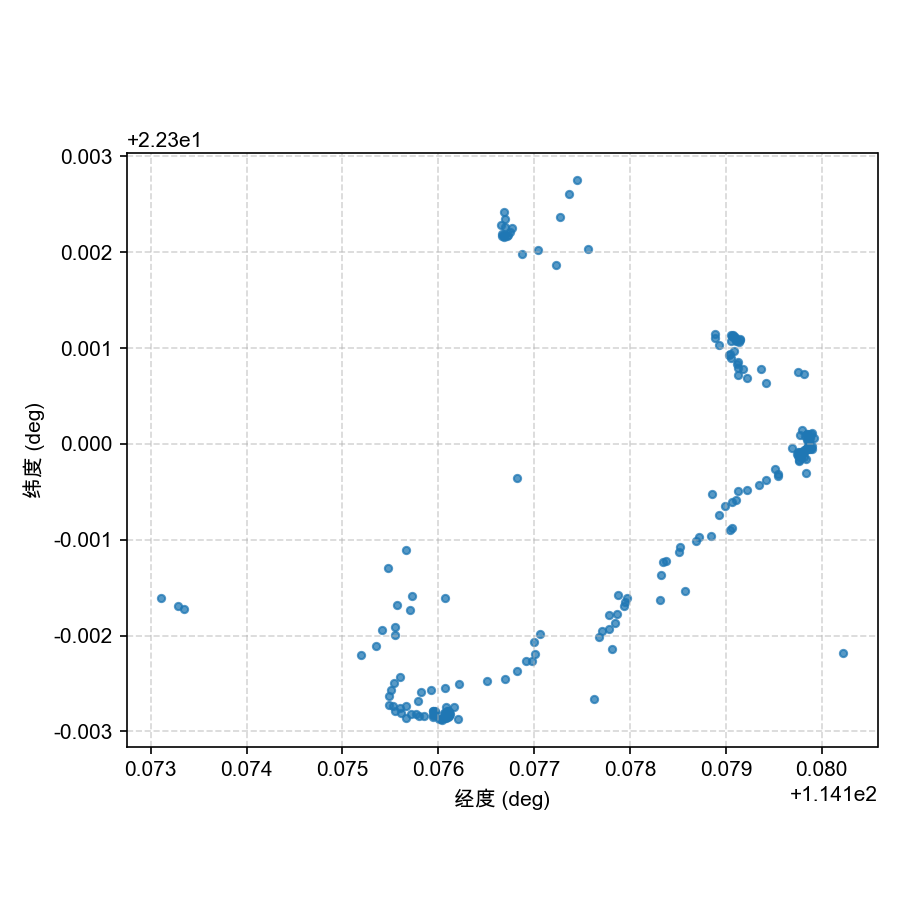
\includegraphics[width=\linewidth]{figures/urban_nav_bds_final/trajectory.png}
\caption*{(b) UrbanNav BDS 轨迹散点图}
\end{minipage}
\caption{UrbanNav 城市动态北斗定位结果}
\end{figure}

\begin{figure}[H]
\centering
\begin{minipage}{0.48\linewidth}
\centering
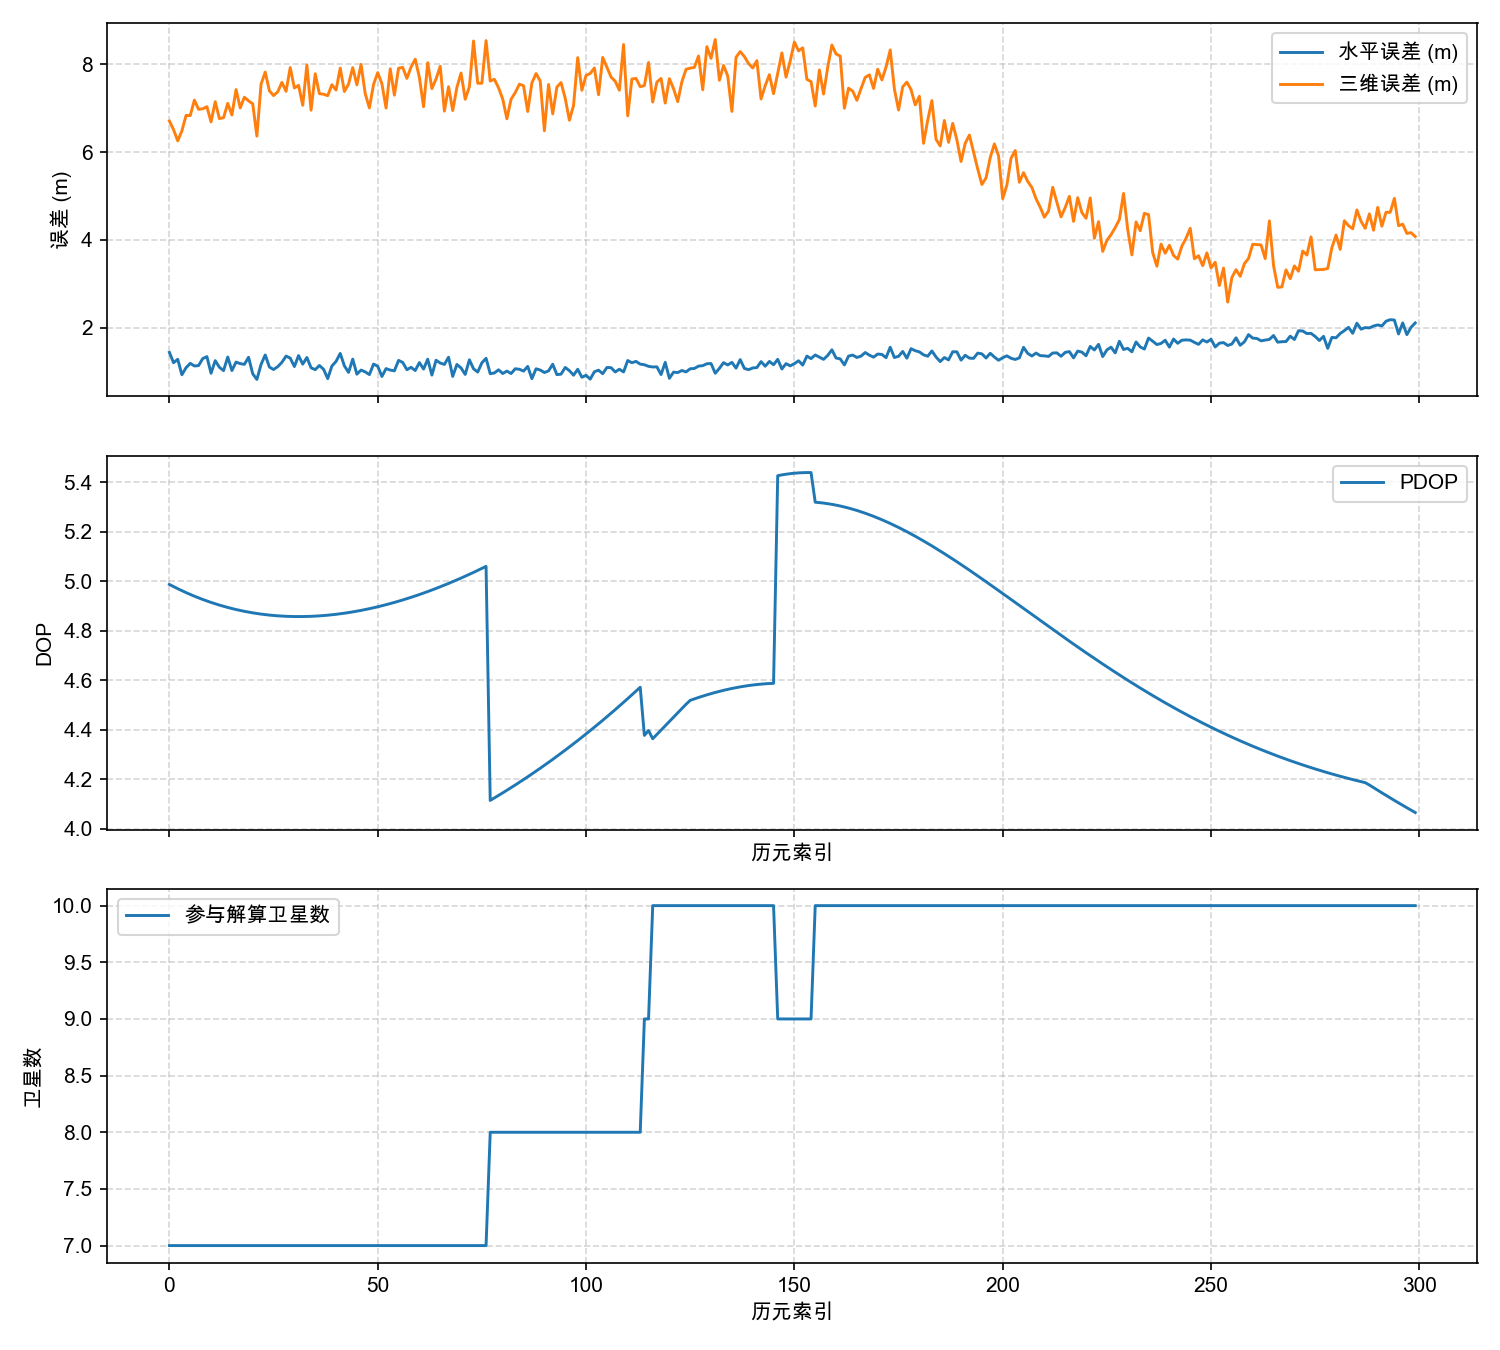
\includegraphics[width=\linewidth]{figures/twtf_bds_final/error_dop.png}
\caption*{(a) TWTF BDS-only 误差曲线}
\end{minipage}
\hfill
\begin{minipage}{0.48\linewidth}
\centering

\includegraphics[width=\linewidth]{figures/twtf_gps_bds_final/error_dop.png}
\caption*{(b) TWTF GPS+BDS 误差曲线}
\end{minipage}
\caption{TWTF 不同系统组合定位结果对比}
\end{figure}

UrbanNav 数据属于城市动态观测场景，北斗单系统定位误差明显大于固定 IGS 站数据，主要与动态接收机、多路径、遮挡和观测环境复杂有关；TWTF 固定站数据中，GPS+BDS 组合解算的 PDOP 低于 BDS-only，三维 RMS 也更小，说明多系统联合能改善卫星几何构型并提升定位稳定性。

\subsubsection{调试问题与解决}

实验过程中主要修复了以下问题：

\begin{itemize}
\item 默认数据路径与实际目录不一致，导致脚本无法开箱运行；已统一为 \texttt{data/sample/}。
\item \texttt{step=0} 会导致除零错误；已在 CLI 和 pipeline 入口增加参数校验。
\item 绘图依赖缺失时仍提示保存成功；已让绘图函数返回状态并由脚本判断。
\item BDS mixed 数据涉及 GPST/BDT 转换和 BDS 电离层参数；已解析 \texttt{BDSA/BDSB} 并修正时间转换。
\item GPS+BDS 共用单一接收机钟差会影响联合解算；已扩展为每系统独立钟差参数。
\item 对不支持的 Hatanaka \texttt{.crx/.d} 文件，程序会给出中文转换提示，避免异常退出。
\end{itemize}

\subsection{结论}

本项目完成了实验基础题要求的五个模块，能够解析 RINEX 数据、计算卫星位置与钟差、进行传播延迟修正、完成伪距单点定位和连续定位分析，并通过 GUI 展示结果。多组数据测试表明，GPS、BDS 和 GPS+BDS 均可稳定运行，能够输出定位结果、误差统计、残差诊断、CSV 文件和可视化图表。

目前系统的特点是模块边界清晰、核心算法手写、支持多系统解算和 GUI 演示。不足之处是观测权重主要基于高度角，尚未充分利用 SNR/CN0；Hatanaka 压缩文件需要外部转换后才能处理。后续可继续加入更丰富的权重模型、长期卫星残差分析和更多站点数据验证。

\subsection{结束语}

通过本次实验，我对卫星导航定位的软件实现过程有了更完整的理解。定位结果并不是单个公式直接给出，而是由数据格式解析、时间系统转换、轨道计算、误差模型和数值解算共同决定。尤其在 BDS 与 GPS mixed 数据中，时间系统、星历选择和系统钟差建模都会显著影响结果。经过多轮调试和测试，项目从单 GPS 样例扩展到 BDS-only 与 GPS+BDS 联合解算，工程可靠性和可演示性都有明显提升。

\subsection{程序清单}

\begin{verbatim}
src/
  analysis.py              误差计算与统计
  atmosphere.py            对流层与电离层改正
  constants.py             物理常数与系统常数
  coords.py                ECEF/BLH/ENU 坐标转换
  experiment_modules.py    五个实验模块封装
  gnss_systems.py          GNSS 系统参数解析与校验
  ml_compensation.py       附加题误差补偿模型
  models.py                核心数据结构
  pipeline.py              连续解算流水线与 CSV 输出
  plot_style.py            中文绘图字体配置
  plotting.py              误差曲线与轨迹散点图
  positioning.py           SPP 加权最小二乘核心
  rinex_nav.py             RINEX 导航文件解析
  rinex_obs.py             RINEX 观测文件解析
  satellite.py             广播星历卫星位置与钟差
  time_utils.py            GPS/BDT 时间工具
scripts/
  gui_app.py               PyQt GUI
  inspect_rinex.py         RINEX 文件检查
  plot_results.py          CSV 结果绘图
  run_batch.py             多数据集汇总
  run_continuous.py        连续定位 CLI
  run_spp.py               单历元定位 CLI
  train_error_model.py     附加题误差模型训练
tests/
  test_experiment_modules.py
\end{verbatim}

\newpage
\appendix
\section{附录：附加题技术实现报告}

\subsection{任务说明与模型选择依据}

附加题要求结合 AI 技术，实现定位误差预测与补偿，并说明模型选择、数据处理、训练细节、补偿步骤、效果验证和改进方向。本项目选择线性回归中的岭回归模型作为误差补偿模型，主要原因如下：

\begin{itemize}
\item 模型结构简单，回归系数具有可解释性，便于分析卫星数、DOP、残差等特征与定位误差之间的关系。
\item 训练样本来自本实验生成的连续定位结果，特征维度较低，线性模型可作为稳定的基准方法。
\item 岭回归在普通最小二乘基础上加入微小正则项，可以减弱特征相关性导致的矩阵病态问题。
\item 为保持项目依赖精简，代码采用项目内手写矩阵方程求解，形式上等价于常见机器学习库中的 Ridge 回归。
\end{itemize}

\subsection{数据处理过程}

模型训练数据来自 6 组连续定位结果，共 17280 条样本，满足“至少 3 组不同场景 RINEX 数据解算结果”的要求。训练脚本读取各数据集的 \texttt{results.csv}，将所有历元结果汇总后，按 70\%/30\% 划分训练集和测试集。

\begin{table}[H]
\centering
\small
\begin{tabular}{lcc}
\toprule
数据来源 & 系统类型 & 样本数 \\
\midrule
BJFS & GPS & 2880 \\
DAEJ & GPS & 2880 \\
HKSL & GPS & 2880 \\
TWTF & GPS & 2880 \\
TWTF & BDS & 2880 \\
TWTF & GPS+BDS & 2880 \\
\bottomrule
\end{tabular}
\caption{附加题训练数据来源}
\end{table}

输入特征选取连续定位结果中与误差相关的解算状态量，包括：

\begin{table}[H]
\centering
\small
\begin{tabular}{p{0.28\linewidth}p{0.62\linewidth}}
\toprule
特征 & 含义 \\
\midrule
\texttt{used\_sats} & 当前历元参与解算的卫星数量，反映观测冗余度。 \\
\texttt{pdop}, \texttt{gdop} & 几何精度因子，反映卫星空间构型对定位误差放大的影响。 \\
\texttt{residual\_rms\_m} & 后验残差 RMS，反映观测噪声和模型误差水平。 \\
\texttt{residual\_max\_m} & 最大后验残差，用于刻画可能存在的粗差或多路径影响。 \\
\texttt{clock\_bias\_m} & 接收机钟差估计值，可间接反映解算状态。 \\
\texttt{h} & 解算高程，高程方向误差对三维定位误差影响明显。 \\
\bottomrule
\end{tabular}
\caption{误差补偿模型输入特征}
\end{table}

预测标签为 ENU 三个方向误差：\texttt{east}、\texttt{north}、\texttt{up}。训练前对输入特征进行均值和标准差归一化，避免不同量纲导致某些特征在法方程中占主导。

\subsection{模型训练细节}

模型实现文件为 \texttt{src/ml\_compensation.py}，训练入口为 \texttt{scripts/train\_error\_model.py}。训练流程如下：

\begin{enumerate}
\item 读取 6 组连续定位 CSV 文件，合并为统一样本表。
\item 使用确定性打乱方式划分训练集和测试集，训练集 12096 条，测试集 5184 条。
\item 计算训练集特征均值与标准差，并对训练集和测试集使用相同参数归一化。
\item 分别对 \texttt{east}、\texttt{north}、\texttt{up} 训练三组岭回归系数。
\item 保存模型参数到 \texttt{results/ml\_compensation/linear\_model.json}，保存指标到 \texttt{metrics.csv}，生成精度对比图。
\end{enumerate}

模型形式为：

\begin{verbatim}
y = beta0 + beta1*x1 + beta2*x2 + ... + betaN*xN
\end{verbatim}

岭回归法方程为：

\begin{verbatim}
(X^T X + lambda I) beta = X^T y
\end{verbatim}

其中偏置项不参与正则化，\texttt{lambda} 取较小值用于增强数值稳定性。线性方程求解使用手写高斯消元，与主项目中“核心算法手写实现”的要求保持一致。

\subsection{补偿实现步骤}

误差补偿流程与原有连续定位结果衔接，具体步骤为：

\begin{enumerate}
\item 原始定位 pipeline 先输出每个历元的坐标、DOP、卫星数、残差和 ENU 误差。
\item 误差模型读取单历元特征并执行 \texttt{model.predict(row)}，得到预测误差 \texttt{pred\_east}、\texttt{pred\_north}、\texttt{pred\_up}。
\item 对原始 ENU 误差进行补偿：
\begin{verbatim}
comp_east  = east  - pred_east
comp_north = north - pred_north
comp_up    = up    - pred_up
\end{verbatim}
\item 根据补偿后的 ENU 误差重新计算水平误差与三维误差。
\item 输出补偿前后 RMS、均值、最大误差，并绘制精度对比图。
\end{enumerate}

当前项目以脚本方式集成该流程：连续定位输出 \texttt{results.csv} 后，训练脚本可自动完成特征读取、模型训练、预测补偿和指标输出。模型参数保存为 JSON，后续可进一步加载到 GUI 或实时 pipeline 中，实现运行过程中的在线误差提示与补偿显示。

\subsection{效果验证与分析}

测试集用于验证补偿效果，评价指标包括水平误差和三维误差的 RMS、均值、最大值。结果如下：

\begin{table}[H]
\centering
\scriptsize
\begin{tabular}{p{0.11\linewidth}p{0.20\linewidth}p{0.21\linewidth}p{0.21\linewidth}p{0.11\linewidth}}
\toprule
数据划分 & 指标 & 原始误差 & 补偿后误差 & 改善率 \\
\midrule
训练集 & 水平 RMS/均值/最大值 & 4.472 / 3.118 / 53.206 & 2.613 / 2.091 / 20.837 & 41.57\% \\
训练集 & 三维 RMS/均值/最大值 & 5.736 / 4.709 / 59.987 & 3.416 / 2.875 / 26.348 & 40.44\% \\
测试集 & 水平 RMS/均值/最大值 & 4.464 / 3.121 / 46.940 & 2.585 / 2.074 / 12.463 & 42.08\% \\
测试集 & 三维 RMS/均值/最大值 & 5.716 / 4.703 / 52.348 & 3.373 / 2.856 / 16.552 & 40.99\% \\
\bottomrule
\end{tabular}
\caption{误差补偿前后精度指标对比，单位为 m}
\end{table}

\begin{figure}[H]
\centering
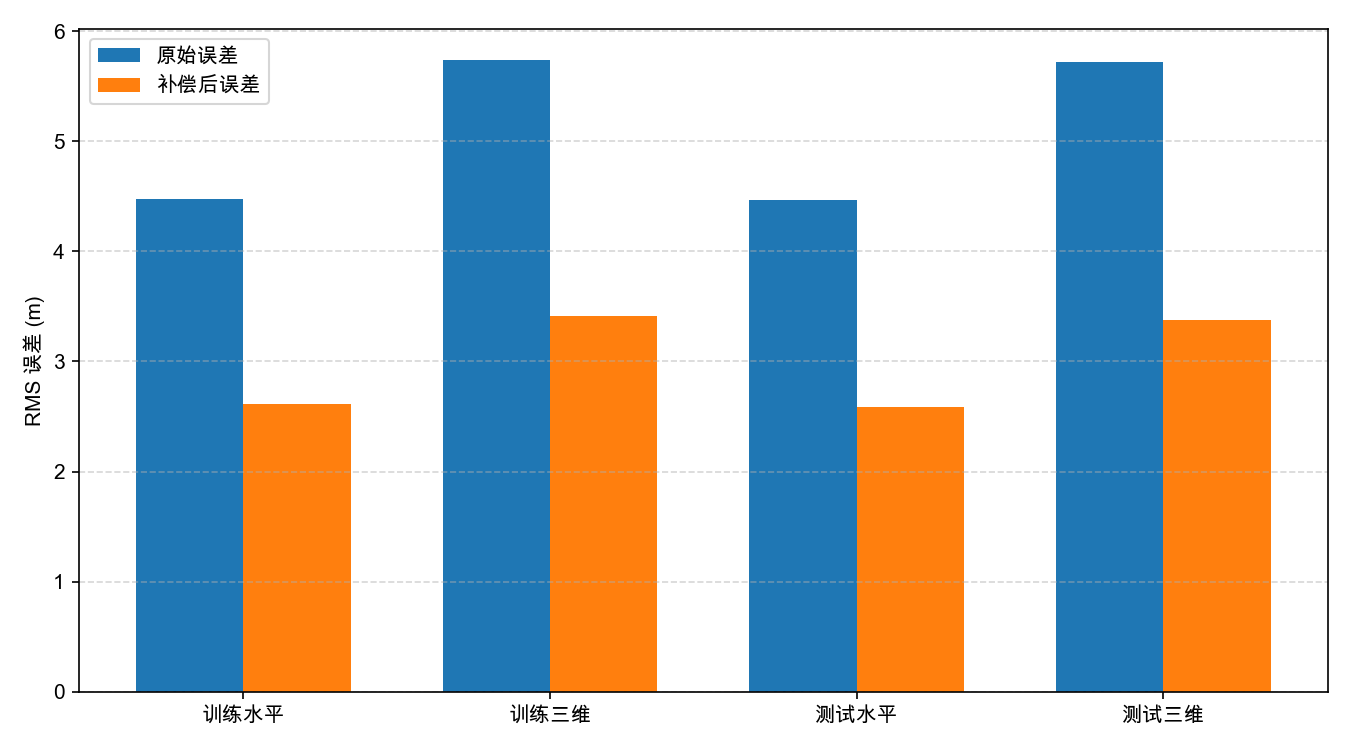
\includegraphics[width=0.60\linewidth]{figures/ml_compensation/compensation_comparison.png}
\caption{误差补偿前后 RMS 对比}
\end{figure}

从结果看，测试集三维 RMS 从 5.716 m 降至 3.373 m，改善率约为 40.99\%；测试集水平 RMS 从 4.464 m 降至 2.585 m，改善率约为 42.08\%。最大误差也明显下降，说明模型能够学习到一部分与 DOP、卫星数、残差和高程相关的系统性误差。

\subsection{优势、不足与改进方向}

线性回归误差补偿的优势是实现简单、运行速度快、参数可解释，适合作为传统 GNSS 解算后的轻量级增强模块。它可以利用定位解算过程中自然产生的 DOP、卫星数量和残差等指标，不需要额外传感器或复杂环境建模。

不足之处在于，线性模型只能表达近似线性关系，对遮挡、多路径、低高度角卫星和不同站点环境差异的非线性影响建模能力有限。此外，当前特征主要来自定位结果 CSV，尚未直接使用每颗卫星的 SNR/CN0、平均高度角、方位角分布等更细粒度信息。

后续改进方向包括：

\begin{itemize}
\item 加入 SNR/CN0、平均高度角、低高度角卫星比例、最大残差卫星等更丰富特征。
\item 使用随机森林或梯度提升树等非线性模型，与线性模型进行对比。
\item 采用跨站点留一验证，检验模型在未知站点上的泛化能力。
\item 将模型加载到 GUI 和连续定位 pipeline 中，实时显示补偿前后定位结果。
\end{itemize}

总体来看，附加题体现了 AI 技术与北斗定位软件开发的融合思路：传统算法负责完成物理模型明确的卫星位置、钟差、延迟修正和最小二乘定位；机器学习模型则利用历史解算结果学习残余误差规律，作为后处理模块进一步提升定位精度。


\end{document}
